% chktex-file 13
% chktex-file 44
% chktex-file 24

\documentclass[../main]{subfiles}

\begin{document}

\subsection{HemeLB}\label{sec:hemelb}

Computational fluid dynamics represents a significant use case for high performance computing in many fields of engineering and science.
Of the many techniques available in this field, the lattice Boltzmann method (LBM) has gained traction in the community for its ability to be both simply deployed for parallel computation and its facility to handle complex geometric and moving boundary conditions.
The HemeLB code\footnote{\url{https://github.com/hemelb-codes}} uses the LBM to study 3D blood flow in human-scale vascular domains and has been optimised to handle the sparse geometries characteristic of these problems.
In previous work, the CPU version of the code has been shown to display strong scaling to over 300,000 cores on SuperMUC-NG~\cite{mccullough2021towards} whilst a GPU port of the code has displayed similar characteristics to over 18,000 NVIDIA V100 GPUs on Summit~\cite{zacharoudiou_development_2022}.

The current GPU ports of HemeLB have been developed using the CUDA framework.
Whilst this has been suitable for the current generations of HPC infrastructure, the imminent arrival of alternative accelerator hardware has necessitated the implementation of more platform-agnostic coding structures.
This effort porting to the OneAPI platform will be instructive as to the level of complexity of such a migration for a mature, detailed and highly performant application.

The OneAPI platform advocates the use of its DPCT conversion tool to convert the majority of an existing CUDA code to the DPC++ framework.
From a practical standpoint, it can be noted that the DevCloud environment that is offered for DPC++ development does not appear to natively contain the CUDA header files necessary for the conversion of an existing CUDA code with DPCT to take place.
As such, conversion needs to be done locally or on a cluster that contains both CUDA and OneAPI software.
Additionally, the majority of resources on the use of DPCT focus on simple, single file, examples of CUDA code.
In reality, porting a mature code will require the conversion and correction of several files to ensure a fully operational application is able to be compiled.
This is further complicated by features such as MPI communication between multiple GPUs.
For the initial porting exercise, we have extracted a single HemeLB collision kernel to test the performance variation between a native CUDA implementation and that converted to DPC++.
The chosen kernel computes the single-relaxation time collision function used by the LBM to solve fluid flow within the simulation domain.
This is used to update the vast majority of sites at each time step and represents the bulk of computation within an iteration.

This kernel was extracted from the main HemeLB code and written into a single CUDA file with appropriate supporting structures and data to allow it to run on a single GPU.
This, highly simplified, script was converted to DPC++ with DPCT.
On our first attempt, the conversion yielded one error that needed to be corrected by hand.
Here it failed to convert a declaration of a constant memory array despite successfully converting several around the same location:

\begin{lstlisting}[language=C++,basicstyle=\small]
dpct::constant_memory<int, 1> _InvDirections_19(19); <--- Converted successfully
//__constant__ double _EQMWEIGHTS_19[19]; <--- Remained after DPCT conversion
dpct::constant_memory<double, 1> _EQMWEIGHTS_19(19); <--- Manually added
dpct::constant_memory<int, 1> _CX_19(19); <--- Converted successfully
\end{lstlisting}

For a updated version of the script, this error no longer occurred.

\subsubsection{Performance Analysis --- Profiling}\label{sec:hemelb_performance}
Following the conversion, we compared the performance of the native CUDA code and the converted code on the NVIDIA A100 GPUs available on the CSD3 cluster.
We also compared this to the Intel GPUs available on the Intel DevCloud environment.
This hardware however should not be regarded as comparable to the A100 cards and these results demonstrate the capacity for cross-platform deployment.
For this test we ran the kernel for the equivalent of 5000 iterations of a 100,000 site domain.
This was repeated 10 times to obtain a fair estimate of the runtime.

\begin{table}[!htbp]
	\begin{tabular}{@{} l l r @{} }
		\toprule
		\thead{Hardware} & \thead{Code} & \thead{Average              runtime (s)} \\
		\midrule
		NVIDIA A100      & CUDA         & \num{0.398578 (0.00020542)}              \\
		NVIDIA A100      & DPC++        & \num{0.4362050 (0.0079303)}              \\
		Intel P630       & DPC++        & \num{15.450100 (0.0939887)}              \\
		\bottomrule
	\end{tabular}
\end{table}

For this initial test case, it can be seen that on the common hardware tested here the conversion to the DPC++ framework and clang compiler has resulted in a 10\% drop in performance compared to the native CUDA code and NVIDIA compiler.

\begin{figure}[htp]
	\centering
	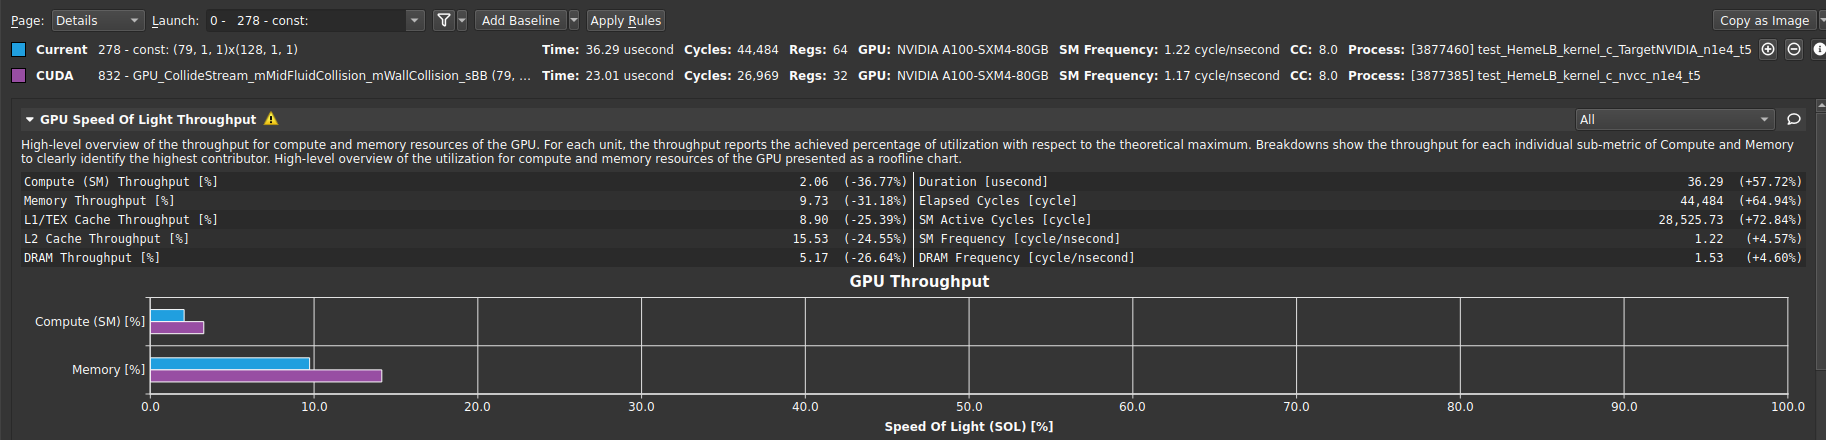
\includegraphics[clip,width=\textwidth]{Nsight_Compute_CUDA_vs_DPC++_A100_GPU.png}
	\caption{Profiling the CUDA and ported DPC++ code using NVIDIA's Nsight Compute on A100 GPU.}
	\label{fig:ncu_CUDA_Vs_DPC++_A100GPU}
\end{figure}

Profiling both versions of the code (CUDA, DPC++) was carried out using NVIDIA's performance analysis tools, Nsight Compute (see fig.~\ref{fig:ncu_CUDA_Vs_DPC++_A100GPU}) and Nsight Systems (see fig.~\ref{fig:nsys_DPC++_A100GPU}).
Nsight Compute provides detailed performance metrics at the kernel level and enables comparison of both versions, although we are not certain about the reliability of the results reported for the DPC++ code.
Nsight Compute reports a 37\% reduction of the compute throughput and a 58\% increase of the kernel's execution time compared to CUDA, while a $\sim10\%$ reduction in overall computational time was reported using either CPU timers (chrono library) or CUDA-specific timers (CUDA event API).
One issue we came across was that the profiler did not return the kernel's name for the DPC++ code.
This information was deducted from the launch statistics (gridsize and blocksize) that matched the corresponding values from profiling the native CUDA code.
The DPC++ ported function (CUDA kernel) is labelled as `const:', instead of the proper kernel's name.


Similar issues are observed with Nsight Systems.
Furthermore, the memory transactions to/from the GPU global memory are reported as memory copies to/from the Host.


\begin{figure}[htp]
	\centering
	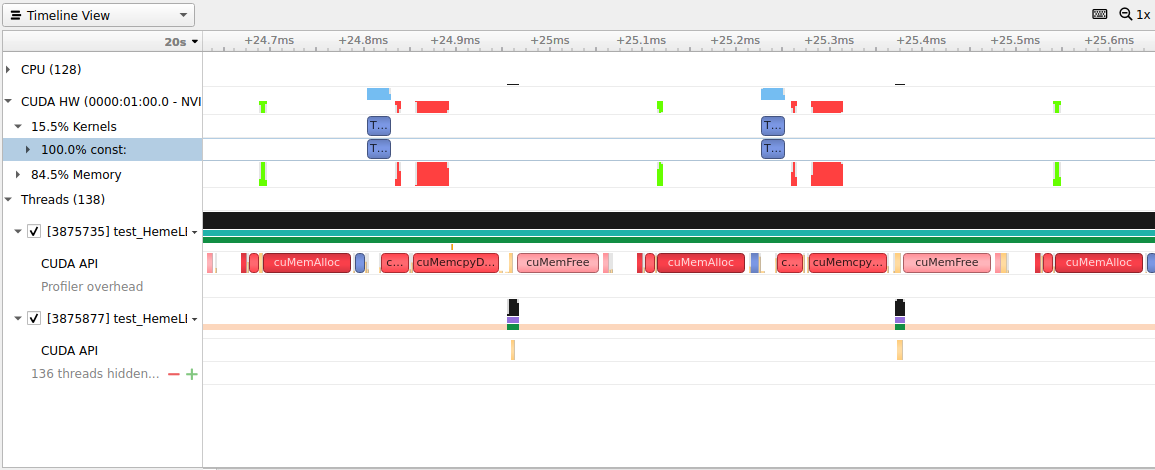
\includegraphics[clip,width=\textwidth]{profile_nsys_DPC++_A100_2steps.png}
	\caption{Profiling the ported DPC++ code using NVIDIA's Nsight Systems on A100 GPU.}
	\label{fig:nsys_DPC++_A100GPU}
\end{figure}

In this initial porting exercise, we have only examined HemeLB's main fluid collision kernel.
With this proof-of-concept completed, the next step would be to work through the full version of the HemeLB code to fully port it to the DPC++ format.
Being a mature code, conducting such a project port will more strongly test the capabilities to effectively port MPI-parallelised CUDA code to the OneAPI framework.


\subsubsection{Porting the full HemeLB\_GPU code}
We further tried porting the full HemeLB\_GPU CUDA code\footnote{\url{https://github.com/UCL-CCS/HemePure-GPU}} to the OneAPI framework on CSD3.
This is a more complex situation, as it involves migrating multiple files to DPC++ and relies on CMake to build and compile the project.

HemeLB relies on a few dependencies (ParMETIS, Boost, CTemplate, TinyXML), which need to be installed prior to compiling the source code.
Hence, one issue that needs to be resolved to ensure fair performance comparison is having the right modules for building/compiling dependencies and native source CUDA code, before repeating the same procedure for the ported DPC++ code.
Whilst HemeLB compilation is generally straightforward, the ease of migration to a new machine is always something of an unknown.

Our workflow on CSD3 was the following:
\begin{enumerate}
	\item Set up modules and the OneAPI environment
	      \begin{verbatim}
module purge
module use /usr/local/software/spack/spack-modules/dpcpp-cuda-20220220/linux-centos8-x86_64_v3/
module load dpcpp
source /usr/local/software/intel/oneapi/2022.1/setvars.sh --force
module load rhel8/slurm dot cmake singularity/current rhel8/global cuda/11.4 /
rhel8/default-amp libtirpc/1.2.6/gcc-9.4.0-duam2pr gcc/9.4.0/gcc-11.2.0-72sgv5z python/3.8.11/gcc-9.4.0-yb6rzr6
    \end{verbatim}
	\item Run DPCT to migrate the full HemeLB\_GPU CUDA code
	\item Compile the DPC++ code
\end{enumerate}


The source files, which specifically contain CUDA code and need to be ported to DPC++ are the following:
\begin{verbatim}
    src
    |- cuda kernels def decl
    ||- GPU Collide Stream Iolets.cu
    ||- GPU Collide Stream wall sBB Iolets.cu
    ||- cuda params.cu
    |
    |- lb
    ||- lb.hpp
    |
    |- net
    ||- BaseNet.cc
    |
    |- Geometry
    ||- LatticeData.cc
    |
    |- main.cu
    |
    |- Simulation Master.cu
\end{verbatim}

In principle, there are two approaches for migrating CUDA codes to DPC++.
The first one involves a file-to-file manual migration, which is a good choice for migrating a few files.
For HemeLB, however, this is not the case.
Hence, we follow an alternative approach, which relies on CMake and passing the compilation database (JSON file) to DPCT for migrating the full project to DPC++.
% For projects using CMake commands it is useful to create a JSON file.
% This will contain the build options of the input project's files, i.e. include path and macros definitions.
The compilation database (compile\_commands.json file), containing the commands required to build the project, is generated by running
\begin{verbatim}
    intercept-build make
\end{verbatim}
%This creates the compile\_commands.json file. %(compilation database containing the commands required to build the project).
%Next running DPCT with the compilation database generates the full ported DPC++ code with a list of warnings that need to be addressed.

The procedure for porting the full HemeLB code is therefore the following:
\begin{enumerate}
	\item Create build directory, e.g. ``src/build''
	\item Within ``src/build'' run ``cmake ..'' % chktex 26
	\item Run ``intercept-build make''. This generates the compilation database (compile\_commands.json)
	\item Navigate one level up (src/).
	\item Run
	      \begin{verbatim}
    dpct -p build/compile_commands.json --in-root=. \
        --out-root=../src_dpct_output --keep-original-code \
        --process-all
    \end{verbatim}
	\item Manually verify and edit the migrated code (in src\_dpct\_output/).
\end{enumerate}

During the migration stage the majority of the warnings received involved CUDA error checking functionalities added in HemeLB\_GPU.
All CUDA runtime API calls return an error code (cudaError\_t is an enum type), while DPC++ uses exceptions to handle errors.
Hence, the tool added messages in the comments to indicate additional manual edits are likely necessary.
For example, warnings were issued for the following in the CUDA code:
\begin{verbatim}
    cudaError_t error = cudaGetLastError();
    cudaError_t cudaStatus;
    cudaStatus = cudaMemcpy(dens_GPU, &(((distribn_t*)GPUDataAddr_dbl_MacroVars)[0]), MemSz, cudaMemcpyDeviceToHost);
    cudaStatus = cudaMalloc((void**)&GPUDataAddr_dbl_MacroVars, TotalMem_dbl_MacroVars);
\end{verbatim}

Warnings were also raised concerning the workgroup size passed to the SYCL ported kernel.
For example:
\begin{verbatim}
    warning: DPCT1049:249: The workgroup size passed to the SYCL kernel
    may exceed the limit. To get the device limit,
    query info::device::max_work_group_size.
    Adjust the workgroup size if needed.
\end{verbatim}

Finally, warnings were also issued for parameters declared in the CUDA code as ``extern''
\begin{verbatim}
    warning: DPCT1057:0: Variable _Iolets_Inlet_Edge was used in host code and
    device code. The Intel(R) DPC++ Compatibility Tool updated _Iolets_Inlet_Edge
    type to be used in SYCL device code and generated
    new _Iolets_Inlet_Edge_host_ct1 to be used in host code. You need to update
    the host code manually to use the new _Iolets_Inlet_Edge_host_ct1.
\end{verbatim}

\subsubsection{Compiling}
We used Intel’s clang++ compiler and passed the flags ``-fsycl'' and ``-fsycl-targets=nvptx64-nvidia-cuda'' to compile SYCL code targeting the NVidia CUDA backend.
One problem detected was that the CMakeLists.txt file was not adjusted accordingly after running the  compatibility tool.
The migrated source files (extension changed to *.dp.cpp) were not updated (in set root\_sources).
In our case this involved the following files:
\begin{verbatim}
./main.dp.cpp
./SimulationMaster.dp.cpp
./geometry/GeometryReader.cc.dp.cpp
./geometry/decomposition/BasicDecomposition.cc.dp.cpp
./colloids/Particle.cc.dp.cpp
./net/BaseNet.cc.dp.cpp
./cuda_kernels_def_decl/GPU_Collide_Stream_Iolets.dp.cpp
./cuda_kernels_def_decl/cuda_params.dp.cpp
./cuda_kernels_def_decl/GPU_Collide_Stream_wall_sBB_Iolets.dp.cpp
./cuda_kernels_def_decl/initialise_GPU.dp.cpp
./extraction/SurfacePointSelector.cc.dp.cpp
./lb/kernels/rheologyModels/CarreauYasudaRheologyModel.cc.dp.cpp
./lb/iolets/InOutLetWomersleyVelocity.cc.dp.cpp
./lb/iolets/InOutLetCosine.cc.dp.cpp
\end{verbatim}

We had to manually modify the following files
\begin{verbatim}
    ./extraction/CMakeLists.txt
    ./geometry/CMakeLists.txt
    ./lb/CMakeLists.txt
    ./net/CMakeLists.txt
    ./colloids/CMakeLists.txt
\end{verbatim}
and modify the CMAKE\_CXX\_FLAGS in the CMakeLists.txt file
\begin{verbatim}
set(CMAKE_CXX_FLAGS "${CMAKE_CXX_FLAGS} -fsycl -fsycl-targets=nvptx64-nvidia-cuda")
\end{verbatim}

We had to adjust the C++ standard to at least 17
\begin{verbatim}
warning: DPCPP does not support C++ version earlier than C++17.
Some features might not be available.
\end{verbatim}

Further compiling problems related to the pow function

\subsubsection{General Comments}
In the first part of this effort, we extracted the key collision kernel of HemeLB into a single script and converted this to DPC++ using the  DPCT conversion tools.
For a code of this level of complexity, The porting and code correction exercise was straightforward even for a developer with limited SYCL experience.

For porting a more complex code such as the CUDA port of HemeLB\_GPU, much more time is needed to understand and complete the conversion process.
As described above, further steps are needed to correctly capture and convert files within a compilation process orchestrated by CMake.
Whilst the documentation describing this process is available, there appear to be fewer examples of such a process compared to single file projects.
It was also noted that using the conversion tool also modified files that did not explicitly contain CUDA code.
As such, a developer choosing to manually convert individual files within a CUDA project may not identify all changes needing to be made to adapt their project to DPC++.

As the conversion to DPC++ makes some fundamental syntactical changes to the converted project files, it does require a user with only a CUDA background to become more familiar with the changes made to the code by the conversion tool and the operation of the SYCL architecture.
The complexity of the converted code will likely govern how much new material must be learnt and modified to achieve a successful port to OneAPI.
This also extends to any compilation errors that arise with the converted code, where dedicated SYCL knowledge may be needed to understand and correct them.
This may be especially true for CUDA functions that do not have direct SYCL equivalents.
For projects with older/legacy code within them, the requirement for a C++17 or above implementation may require further developer effort to ensure a successful conversion.

Generally speaking however, we note that the warnings are clear and running the  compatibility tool for porting the full CUDA HemeLB\_GPU code is straightforward.
This makes the porting process a task that even a developer with little to no experience in SYCL can carry out.

\subsubsection{Estimate of Development Effort}
Based on the effort conducted at the time of writing this report we would estimate that roughly 3 months FTE (i.e.\ dedicated work) would be required to fully convert the HemeLB\_GPU from CUDA to the OneAPI platform.
This estimate was made based on developers having no prior experience with OneAPI or SYCL prior to this exercise.
Unsupported developers from the same background may take longer.
As the conversion to OneAPI invokes more fundamental code changes than some other GPU porting approaches (e.g.\ with HIP) it does demand the developer to gain more understanding of the SYCL and OneAPI programming approaches and the differences to CUDA.
At the time of writing, a detailed performance comparison of the ported and CUDA version of the full HemeLB\_GPU had not been able to be made.
Further developer time would be required to further tune the ported version of the code to minimise performance losses compared to the native CUDA version.

\end{document}
